% Aux A + Aux B — STE forward/backward + XOR/popcount deployment equivalent.
% Full-width standalone. Compile:  pdflatex arch_expand_aux.tex

\documentclass[tikz,border=8pt]{standalone}
\usepackage{tikz}
\usepackage{amsmath,amssymb}
\usepackage{xcolor}
\usetikzlibrary{positioning,arrows.meta,calc,fit,backgrounds}

\newcommand{\bV}{\mathbf{V}}
\newcommand{\bipset}{\{-1,+1\}}

\definecolor{cBipolar}{HTML}{2C5282}
\definecolor{cAux}{HTML}{276749}
\definecolor{cPanelBg}{HTML}{FAFBFC}
\definecolor{cPanelBorder}{HTML}{CBD5E0}

\tikzset{
  block/.style={draw=cPanelBorder, fill=cPanelBg, thick, rounded corners=6pt,
                inner sep=8pt, minimum width=170mm},
  blockTitle/.style={font=\bfseries\normalsize, anchor=north west, inner sep=6pt},
  cellPlain/.style={draw=black!30, fill=white, font=\small\ttfamily,
                    minimum width=8mm, minimum height=7mm, inner sep=0pt},
  lbl/.style={font=\scriptsize\itshape, text=black!65, align=center},
  subHead/.style={font=\small\bfseries, anchor=south west},
}

\begin{document}
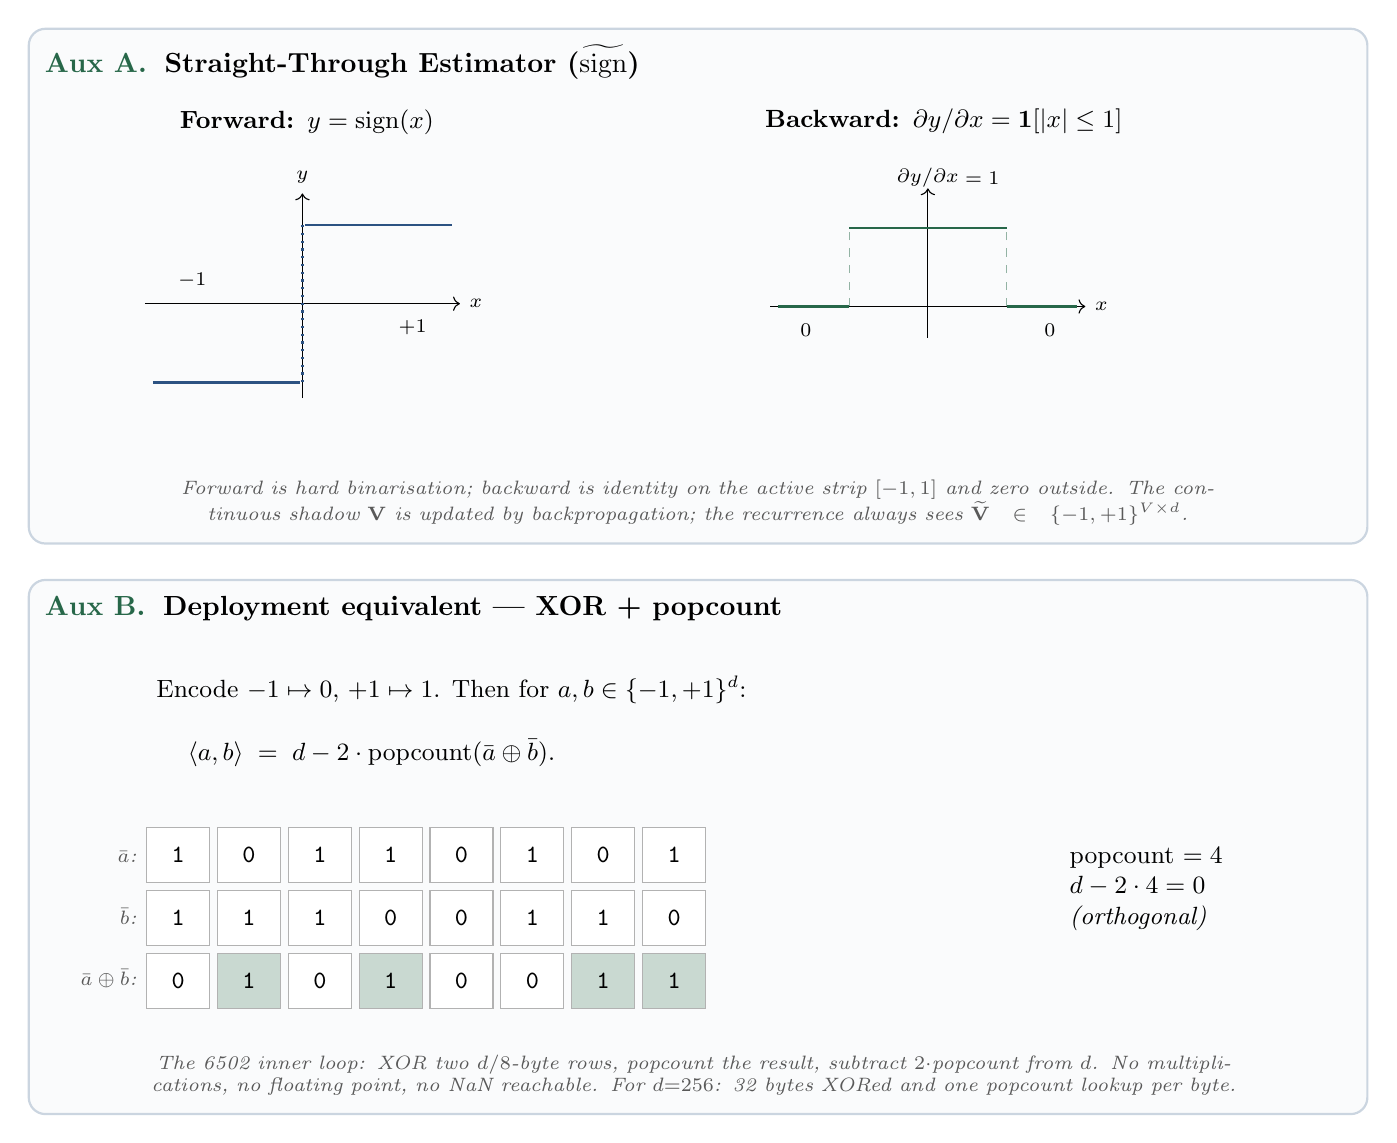
\begin{tikzpicture}

% ========== AUX A: STE ==========
\node[block, minimum height=186pt, anchor=north west] (AA) at (-0.01,1.01) {};
\node[blockTitle] at (AA.north west)
  {\textcolor{cAux}{Aux A.}\;\;Straight-Through Estimator ($\widetilde{\mathrm{sign}}$)};

% forward plot (left)
\begin{scope}[shift={(99pt,-71pt)}]
  \node[subHead] at (-1.68, 2.02) {Forward: $y = \mathrm{sign}(x)$};
  \draw[->] (-2.0,0) -- (2.0,0) node[right, font=\scriptsize] {$x$};
  \draw[->] (0,-1.2) -- (0,1.4) node[above, font=\scriptsize] {$y$};
  \draw[thick, cBipolar] (-1.9,-1) -- (-0.03,-1);
  \draw[thick, cBipolar] (0.03, 1) -- ( 1.9, 1);
  \draw[thick, cBipolar, dotted] (0,-1) -- (0,1);
  \node[font=\scriptsize] at (1.4,-0.3) {$+1$};
  \node[font=\scriptsize] at (-1.4,0.3) {$-1$};
\end{scope}

% backward plot (right)
\begin{scope}[shift={(325pt,-72pt)}]
  \node[subHead] at (-2.19, 2.07) {Backward: $\partial y/\partial x = \mathbf{1}[|x|\le 1]$};
  \draw[->] (-2.0,0) -- (2.0,0) node[right, font=\scriptsize] {$x$};
  \draw[->] (0,-0.4) -- (0,1.5) node[above, font=\scriptsize, pos=0.94] {$\partial y/\partial x$};
  \draw[thick, cAux] (-1.9,0) -- (-1.0,0);
  \draw[thick, cAux] (-1.0,1) -- (1.0, 1);
  \draw[thick, cAux] (1.0, 0) -- (1.9, 0);
  \draw[dashed, cAux!50] (-1.0,0) -- (-1.0,1);
  \draw[dashed, cAux!50] ( 1.0,0) -- ( 1.0,1);
  \node[font=\scriptsize, anchor=south] at (0.69,1.42) {$= 1$};
  \node[font=\scriptsize] at (-1.55,-0.3) {$0$};
  \node[font=\scriptsize] at ( 1.55,-0.3) {$0$};
\end{scope}

\node[lbl, align=center, text width=155mm, anchor=south]
  at (8.5, -5.44)
  {Forward is hard binarisation; backward is identity on the active strip
   $[-1,1]$ and zero outside. The continuous shadow $\bV$ is updated by
   backpropagation; the recurrence always sees
   $\widetilde\bV \in \bipset^{V\times d}$.};

% ========== AUX B: XOR/POPCOUNT ==========
\node[block, minimum height=193pt, anchor=north west] (AB) at (-0.01,-5.99) {};
\node[blockTitle] at (AB.north west)
  {\textcolor{cAux}{Aux B.}\;\;Deployment equivalent --- XOR + popcount};

\begin{scope}[shift={(1.5,-7.4)}]
  \node[font=\small, anchor=west] at (0, 0)
    {Encode $-1\mapsto 0$, $+1\mapsto 1$. Then for $a,b\in\bipset^d$:};
  \node[font=\small, anchor=west] at (0.4, -0.8)
    {$\langle a,b\rangle \;=\; d - 2\cdot\mathrm{popcount}(\bar a \oplus \bar b).$};

  \begin{scope}[shift={(0.4,-2.1)}]
    \node[lbl, anchor=east] at (-0.4, -0.02) {$\bar a$:};
    \foreach \v [count=\i from 0] in {1,0,1,1,0,1,0,1}
      \node[cellPlain] at (\i*0.9, 0) {\v};

    \node[lbl, anchor=east] at (-0.4, -0.78) {$\bar b$:};
    \foreach \v [count=\i from 0] in {1,1,1,0,0,1,1,0}
      \node[cellPlain] at (\i*0.9, -0.8) {\v};

    \node[lbl, anchor=east] at (-0.4, -1.57) {$\bar a\oplus\bar b$:};
    \foreach \v [count=\i from 0] in {0,1,0,1,0,0,1,1} {
      \ifnum\v=1
        \node[cellPlain, fill=cAux!25] at (\i*0.9, -1.6) {\v};
      \else
        \node[cellPlain] at (\i*0.9, -1.6) {\v};
      \fi
    }

    \node[font=\small, anchor=west, align=left] at (11.2, -0.43)
      {popcount $= 4$\\
       $d - 2\cdot 4 = 0$\\
       \emph{(orthogonal)}};
  \end{scope}
\end{scope}

\node[lbl, align=center, text width=155mm, anchor=south]
  at (8.45, -12.67)
  {The 6502 inner loop: XOR two $d/8$-byte rows, popcount the result,
   subtract $2\cdot$popcount from $d$. No multiplications, no floating
   point, no NaN reachable. For $d{=}256$: 32 bytes XORed and one
   popcount lookup per byte.};

\end{tikzpicture}
\end{document}
